En esta sección, realizaremos diversos experimentos para verificar tanto el tiempo de ejecución como la calidad de las soluciones de nuestro algoritmo de búsqueda local.

Como dijimos anteriormente, el algoritmo de búsqueda local toma una solución inicial. Nosotros tomamos como un parámetro del algoritmo la solución inicial que éste recibe.

En los gráficos que presentamos a continuación, mostramos el tiempo de ejecución de correr búsqueda local con dos algoritmos que nos dan soluciones iniciales. Un algoritmo es el algoritmo goloso que detallamos en la sección \ref{subsub:algoritmos-heuristicos-goloso-desarrollo.tex}, y el otro es el algoritmo de Dijkstra tomando como pesos de las aristas la función $\omega_1$.

\begin{figure}[H]
  \begin{minipage}{0.5\linewidth}
    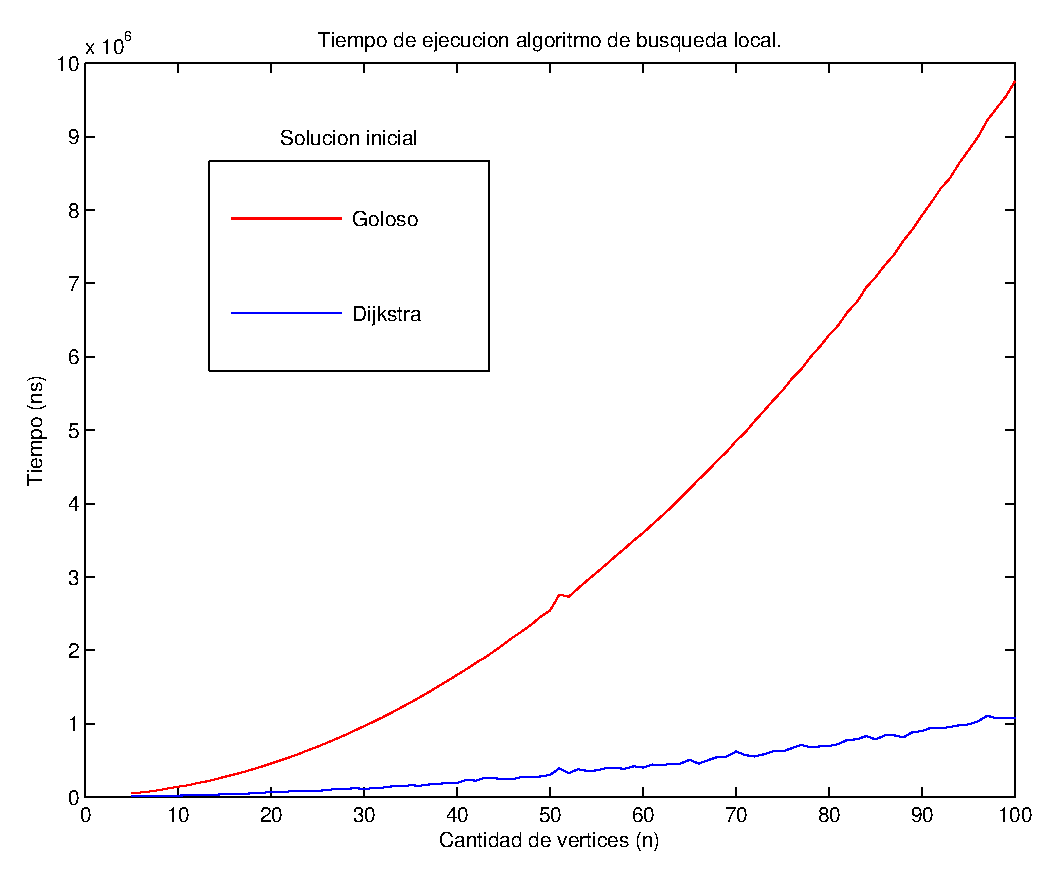
\includegraphics[width=\linewidth]{graficos/busq_local_tiempo.eps}
    \caption{Tiempo ejecución búsqueda local}\label{fig:busq-local-tiempo}
  \end{minipage}
  \hfill
  \begin{minipage}{0.5\linewidth}
    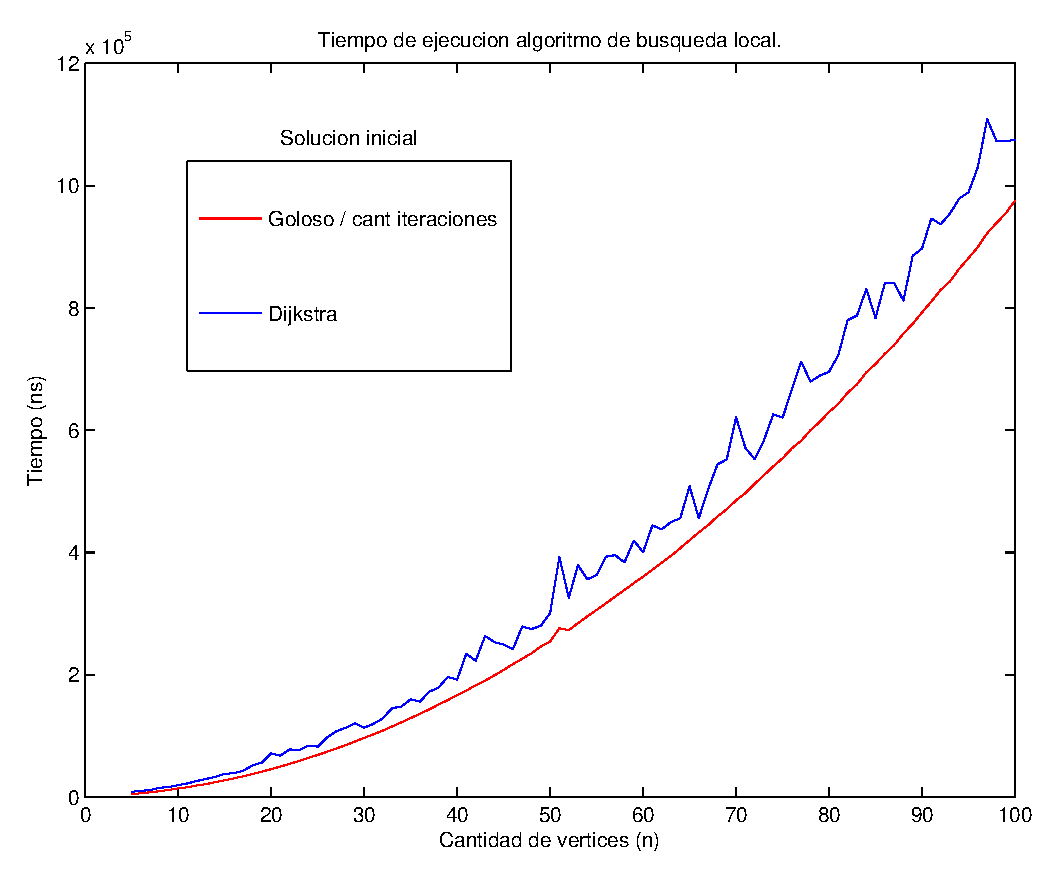
\includegraphics[width=\linewidth]{graficos/busq_local_tiempo_divido10.eps}
    \caption{Idem divido 10}\label{fig:busq-local-tiempo-div10}
  \end{minipage}
\end{figure}

Como podemos observar en el gráfico \ref{fig:busq-local-tiempo} el algoritmo de búsqueda local utilizando nuestro algoritmo goloso tiene un tiempo de ejecución mayor al que utiliza el algoritmo de Dijkstra. Esto se debe a que lo que medimos es el tiempo en correr primero los algoritmos que generan las soluciones iniciales y luego correr el algoritmo de búsqueda local. Como ya sabemos nuestro algoritmo goloso corre el algoritmo de Dijkstra una cantidad de iteraciones prefijada. Resulta lógico pensar que un algoritmo que corre el algoritmo de Dijkstra muchas veces tendrá un tiempo de ejecución mayor al de un algoritmo que lo corre sólo una.

Por esto en el gráfico \ref{fig:busq-local-tiempo-div10} mostramos los mismos tiempos que en el otro gráfico pero dividimos el tiempo que tarda el algoritmo de búsqueda local que usa nuestro algoritmo goloso por \emph{cant iteraciones}. Con este gráfico, logramos ver que el tiempo de ejecución de ambos algoritmos de búsqueda es parecido cuando reducimos el factor de tiempo de ejecución del algoritmo nos da la solución inicial.

A continuación incluimos unos gráficos que comparan la calidad de las soluciones del algoritmo de búsqueda local.

\begin{figure}[H]
  \begin{minipage}{0.5\linewidth}
    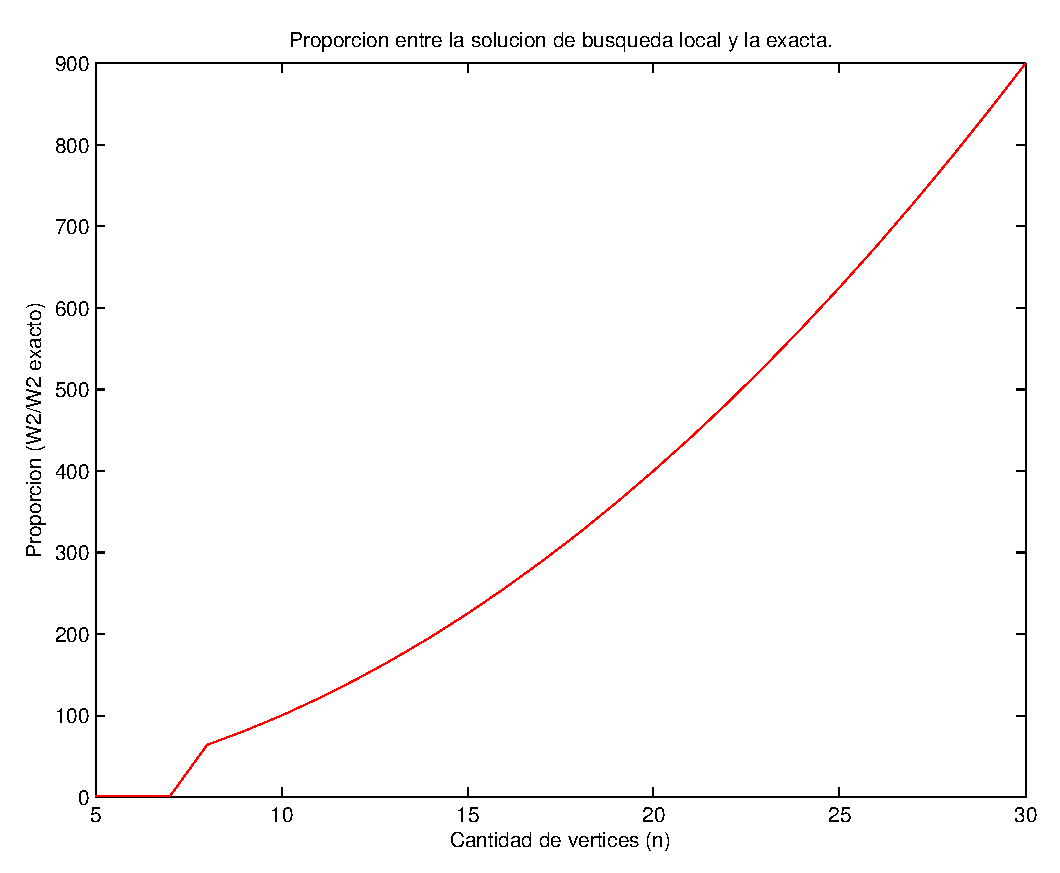
\includegraphics[width=\linewidth]{graficos/busq_local_proporcion.eps}
    \caption{Diferencia proporcional busqueda/exacto}\label{fig:busq-local-proporcion}
  \end{minipage}
  \hfill
  \begin{minipage}{0.5\linewidth}
    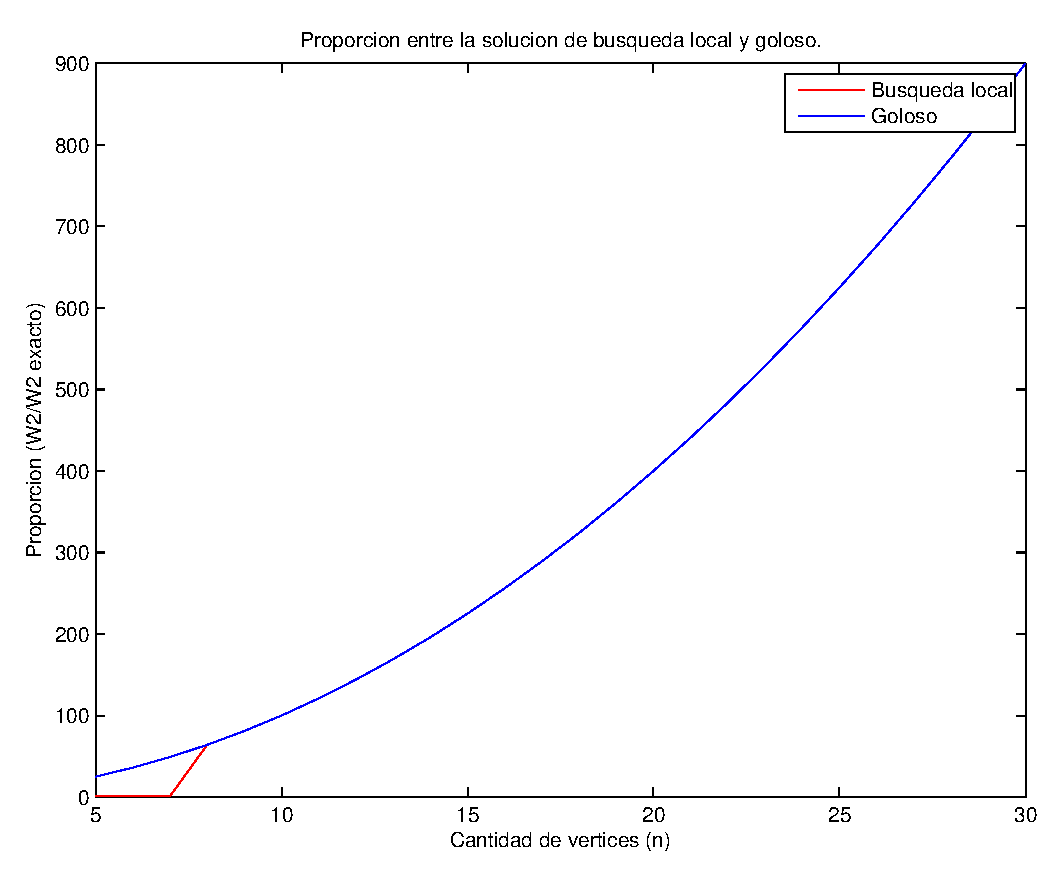
\includegraphics[width=\linewidth]{graficos/busq_local_proporcion_comparacion.eps}
    \caption{Calidad Soluciones Goloso/Dijkstra}\label{fig:busq-local-proporcion-comparacion}
  \end{minipage}
\end{figure}

El gráfico \ref{fig:busq-local-proporcion} muestra la diferencia proporcional entre las soluciones que nos da el algoritmo de búsqueda local con una solución inicial dada por nuestro algoritmo goloso y el algoritmo exacto para la familia de grafos que rompe nuestro algoritmo goloso. El gráfico de la Figura \ref{fig:busq-local-proporcion-comparacion} compara la proporción con respecto al algoritmo exacto de las soluciones dadas por el algoritmo goloso y las soluciones resultantes de aplicar búsqueda local tomando como soluciones iniciales a las soluciones dadas por el algoritmo goloso para la misma familia de grafos del gráfico de la Figura \ref{fig:busq-local-proporcion}. Mostramos esto en dos gráficos distintos para que se logre apreciar que para la mayoría de los casos, el algoritmo de búsqueda local no logra mejorar las soluciones del nuestro algoritmo goloso para esta familia.

Vale aclarar que en este experimento pudimos correr el algoritmo exacto para grafos con una cantidad de nodos un poco mayor que en las anteriores mediciones. Esto se debe a que para esta familia de grafos el algoritmo exacto tarda menos tiempo en correr ya que hay menos caminos que revisar (recordemos que los grafos de nuestra familia se componen de tres caminos disjuntos en aristas).

Como podemos observar para $n = 5$ nuestro algoritmo de búsqueda local logra mejorar la calidad de las soluciones dadas por nuestro algoritmo goloso. Esto es porque para un dicho valor de $n$ el grafo se compone de tres caminos de $3$ nodos cada uno, los cuales comparten los nodos de los extremos pero no el nodo del medio. Debido a esto, estos tres caminos son vecinos entre sí para nuestra vecindad, ya que se puede por ejemplo cambiar el nodo del medio de uno de los caminos para pasar a otro utilizando la operación de Cambiar Nodo definida en la sección \ref{subsub:algoritmos-heuristicos-busqueda-desarrollo_vecindad.tex}. Por lo tanto al correr el algoritmo de búsqueda local, éste puede devolver como solución el mejor de estos $3$ caminos.

Sin embargo, cuando $n > 5$ los tres caminos del grafo dejan de tener 3 nodos pero siguen teniendo en común sólo a sus extremos, por lo tanto no son vecinos entre sí para nuestra vecindad. Por este motivo el algoritmo de búsqueda local no puede mejorar la solución inicial dada por nuestro algoritmo goloso ya que ésta no tiene vecinos.

A continuación incluiremos un gráfico que compara la calidad de las soluciones del algoritmo de busqueda local cuando éste toma como solución inicial la dada por el algoritmo de Dijkstra tomando como función de peso el para las aristas la función $\omega_1$

\begin{figure}[H]
  \begin{minipage}{0.5\linewidth}
    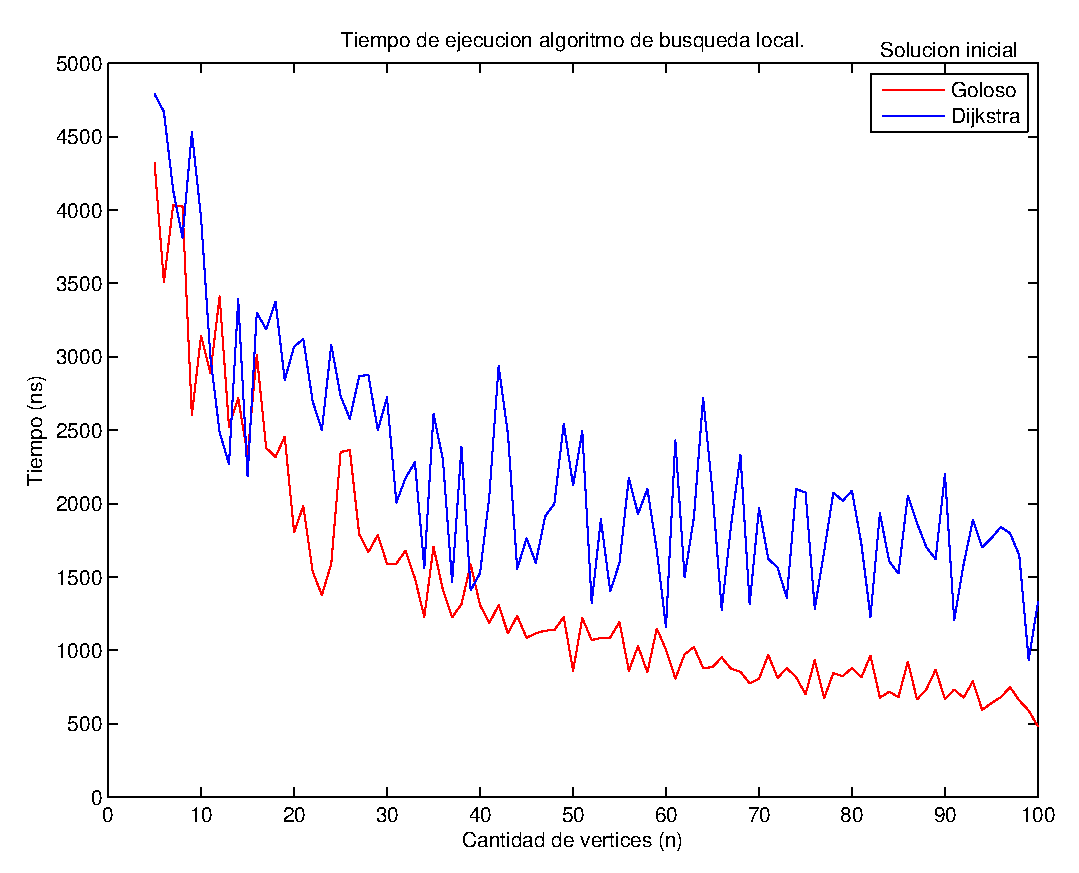
\includegraphics[width=\linewidth]{graficos/busq_local_calidad.eps}
    \caption{Diferencia proporcional busqueda/exacto}\label{fig:busq-local-calidad}
  \end{minipage}
\end{figure}
  
Como podemos observar en la Figura \ref{fig:busq-local-calidad}, para los grafos con los que hicimos las mediciones, el algoritmo que toma como solución inicial la dada por nuestro algoritmo goloso en general es mejor que la dada por el algoritmo de Dijkstra.

%TODO decir porque es mejor con el goloso
%Creemos que esto es así porque, como ya vimos en la sección \ref{subsub:algoritmos-heuristicos-goloso-experimentacion.tex} las soluciones dadas por nuestro algoritmo goloso son mejores que las dadas por el algoritmo de Dijkstra. Una vez que nuestro algoritmo de búsqueda local toma estas soluciónes iniciales las mejora pero no las logra mejorar lo suficiente como para que las soluciones que da Dijkstra supere a las que da nuestro algoritmo goloso.